\HydraSection[
  focus x=0.65,
  focus y=0.57,
  radius=0.14,
  zoom=1.85
]{Growth, injury \& source density}


% -----------------------------------------------------------------------------
% Live experiment 1: a local activator perturbation on a short domain
% -----------------------------------------------------------------------------
\begin{frame}{Can a local activator perturbation create a second organizer?}

  \vspace{-0.18cm}

  \begin{columns}[c,onlytextwidth]
    \begin{column}{0.47\textwidth}
      {\color{HydraGold}\bfseries\fontsize{7.7}{9.2}\selectfont
        THE LIVE EXPERIMENT\par}

      \vspace{0.16cm}

      \HydraPoint[HydraGold]
        {Begin with one organizer}
        {A stable peak is already established on the short domain.}

      \vspace{-0.12cm}

      \HydraPoint[HydraCyan]
        {Add activator locally}
        {A brief, localized perturbation creates a second candidate peak away from the first.}

      \vspace{-0.12cm}

      \HydraPoint[HydraRed]
        {Then release the system}
        {After the perturbation, the autonomous nonlinear dynamics select the outcome.}
    \end{column}

    \begin{column}{0.49\textwidth}
      {\color{HydraMuted}\bfseries\fontsize{7.7}{9.2}\selectfont
        WHAT COULD HAPPEN?\par}

      \vspace{0.16cm}

      \HydraPoint[HydraGold]
        {A second organizer forms}
        {The added peak becomes self-maintaining and both organizers persist.}

      \vspace{-0.12cm}

      \HydraPoint[HydraRed]
        {The added peak disappears}
        {It remains transient, loses the competition and the original one-peak pattern returns.}
    \end{column}
  \end{columns}

  \vspace{0.22cm}

  \begin{center}
    {\color{HydraWhite}\bfseries\fontsize{12.5}{15.3}\selectfont
      Does local activation create a new organizer --- or only a transient peak?
    \par}
  \end{center}
\end{frame}


\begin{frame}{The small domain cannot sustain a second peak}

  \vspace{-0.14cm}

  \begin{columns}[c,onlytextwidth]
    \begin{column}{0.47\textwidth}
      {\color{HydraGold}\bfseries\fontsize{7.7}{9.2}\selectfont
        OBSERVED IN THE LIVE SIMULATION\par}

      \vspace{0.14cm}

      \HydraPoint[HydraGold]
        {The original peak persists}
        {The established organizer remains self-maintaining.}

      \vspace{-0.12cm}

      \HydraPoint[HydraRed]
        {The added peak decays}
        {The local activator perturbation does not become a second organizer.}
    \end{column}

    \begin{column}{0.49\textwidth}
      {\color{HydraCyan}\bfseries\fontsize{7.7}{9.2}\selectfont
        NONLINEAR INTERPRETATION\par}

      \vspace{-0.12cm}

      {\color{HydraWhite}\fontsize{10.2}{13}\selectfont
      \begin{align*}
        (\bar u_1,\bar v_1)+(\delta u,0)
        \quad\longrightarrow\quad
        (\bar u_1,\bar v_1).
      \end{align*}
      }

      \vspace{-0.32cm}

      \HydraPoint[HydraCyan]
        {Competition through inhibition}
        {The broad inhibitor field couples the two candidate peaks.}

      \vspace{-0.12cm}

      \HydraPoint[HydraGold]
        {Limited spatial capacity}
        {For these parameters, $[0,1]$ supports the one-peak attractor but not two persistent organizers.}
    \end{column}
  \end{columns}

  \vspace{0.02cm}

  \HydraTakeaway{
    A local activator perturbation need not enter the basin of a new spatial pattern
  }
\end{frame}


% -----------------------------------------------------------------------------
% Live experiment 2: diffusion-driven instability on a larger fixed domain
% -----------------------------------------------------------------------------
\begin{frame}{Does a larger Hydra necessarily grow more heads?}

  \vspace{-0.16cm}

  \begin{columns}[c,onlytextwidth]
    \begin{column}{0.47\textwidth}
      {\color{HydraGold}\bfseries\fontsize{7.7}{9.2}\selectfont
        MORE SPACE CHANGES WHAT CAN FIT\par}

      \vspace{0.16cm}

      \HydraPoint[HydraGold]
        {Peaks can separate}
        {A longer domain creates regions farther from the existing organizer.}

      \vspace{-0.12cm}

      \HydraPoint[HydraCyan]
        {More structures are possible}
        {Several well-separated activator peaks may now coexist.}

      \vspace{-0.12cm}

      \HydraPoint[HydraRed]
        {Large fixed-domain experiment}
        {Starting from a nearly uniform state with noise can produce many peaks.}
    \end{column}

    \begin{column}{0.49\textwidth}
      {\color{HydraMuted}\bfseries\fontsize{7.7}{9.2}\selectfont
        BUT OUR HYDRA ALREADY HAS ONE HEAD\par}

      \vspace{0.16cm}

      \HydraPoint[HydraGold]
        {The initial state is different}
        {Growth begins from an established organizer, not from uniform noise.}

      \vspace{-0.12cm}

      % \HydraPoint[HydraCyan]
      %   {The existing pattern has memory}
      %   {The organizer and its inhibitor field influence where another peak can form.}

      \vspace{-0.12cm}

      \HydraPoint[HydraRed]
        {The real question}
        {As the domain grows, will one head persist, split or generate additional heads?}
    \end{column}
  \end{columns}

  \vspace{0.14cm}

  \HydraTakeaway{
    A larger domain permits more peaks, growth determines whether they appear
  }
\end{frame}


% -----------------------------------------------------------------------------
% Live experiment 3: the same growth endpoint reached at different rates
% -----------------------------------------------------------------------------
\begin{frame}{Growth selects number of peaks}

  \vspace{-0.18cm}

  \begin{center}
    {\color{HydraWhite}\bfseries\fontsize{12.4}{15.5}\selectfont
      Let $\Omega$ grow in time: $\Omega(t)=[0,L(t)]$.
    \par}
  \end{center}

  \vspace{0.18cm}

  \begin{columns}[T,onlytextwidth]
    \begin{column}{0.47\textwidth}
      {\centering\color{HydraCyan}\bfseries\fontsize{12}{14.5}\selectfont
        SLOW GROWTH\par}

      \vspace{0.14cm}

      {\centering\color{HydraWhite}\fontsize{10.4}{12.8}\selectfont
        The domain length changes gradually.
      \par}

      \vspace{0.18cm}

      {\centering\color{HydraBody}\fontsize{8.2}{10.3}\selectfont
        the solution has time to reorganize as successive modes become available
      \par}
    \end{column}

    \begin{column}{0.47\textwidth}
      {\centering\color{HydraGold}\bfseries\fontsize{12}{14.5}\selectfont
        FAST GROWTH\par}

      \vspace{0.14cm}

      {\centering\color{HydraWhite}\fontsize{10.4}{12.8}\selectfont
        The domain length changes rapidly.
      \par}

      \vspace{0.18cm}

      {\centering\color{HydraBody}\fontsize{8.2}{10.3}\selectfont
        the domain crosses the same instability ranges on a different timescale
      \par}
    \end{column}
  \end{columns}

  \vspace{0.52cm}

  \begin{center}
    {\color{HydraGold}\bfseries\fontsize{13.0}{15.8}\selectfont
      Same initial organizer. Same final length. Same final pattern?
    \par}
  \end{center}

  \vspace{0.10cm}

  \HydraTakeaway{
    The growth rate becomes a nonlinear pattern-selection parameter
  }
\end{frame}


% -----------------------------------------------------------------------------
% Live experiment 4: remove the head but omit the biological wound response
% -----------------------------------------------------------------------------
\HydraSubsection[
  \mbox{A cut changes the geometry,}
  \mbox{but regeneration also requires}
  \mbox{an injury-induced signal}
]{Role of the wound}


\begin{frame}{Is removing the head enough to trigger regeneration?}

  \vspace{-0.16cm}

  \begin{columns}[c,onlytextwidth]
    \begin{column}{0.49\textwidth}
      {\color{HydraGold}\bfseries\fontsize{7.7}{9.2}\selectfont
        WHAT THE LIVE MODEL DOES\par}

      \vspace{0.16cm}

      \HydraPoint[HydraGold]
        {Head removed}
        {The part of the simulated domain containing the organizer is discarded.}

      \vspace{-0.12cm}

      \HydraPoint[HydraCyan]
        {Profiles inherited}
        {The remaining fragment keeps the activator and inhibitor profiles present before the cut.}

      \vspace{-0.12cm}

      \HydraPoint[HydraRed]
        {Wound response omitted}
        {The geometry changes, but no additional biological signal is introduced.}
    \end{column}

    \begin{column}{0.47\textwidth}
      {\centering\color{HydraMuted}\fontsize{7.6}{9.2}\selectfont
        LIVE OUTCOME\par}

      \vspace{0.26cm}

      {\centering\color{HydraWhite}\bfseries\fontsize{13.2}{16}\selectfont
        THE HEAD DOES NOT REGROW
      \par}

      \vspace{0.34cm}

      \HydraPoint[HydraRed]
        {The residual signal fades}
        {The inherited headless profile relaxes toward the zero state.}

      \vspace{-0.12cm}

      \HydraPoint[HydraGold]
        {No organizer is initiated}
        {Nothing pushes the fragment into the basin of a head-forming pattern.}
    \end{column}
  \end{columns}

  \vspace{0.06cm}

  \HydraTakeaway{
    Changing the geometry is not the same as activating a wound response
  }
\end{frame}


% -----------------------------------------------------------------------------
% Biological evidence: head loss with and without tissue injury
% -----------------------------------------------------------------------------
\begin{frame}{How the head is removed determines whether it regenerates}

  \vspace{-0.10cm}

  \begin{columns}[c,onlytextwidth]
    \begin{column}{0.62\textwidth}
      \centering
      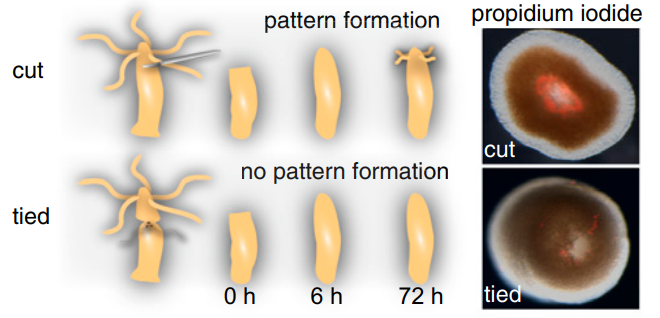
\includegraphics[
        width=\linewidth,
        height=5.00cm,
        keepaspectratio
      ]{figures/E_growth_wound_and_sd/WoundRole.png}
      
      \vspace{0.04cm}

      {\color{HydraMuted}\fontsize{6}{7.2}\selectfont
      Tursch et al.,
      \textit{PNAS}
      119, e2204122119 (2022), Fig.~1A.\par
      }
    \end{column}

    \begin{column}{0.34\textwidth}
      \HydraPoint[HydraRed]
        {Cut: wound present}
        {Cutting disrupts epithelial integrity. Pattern formation follows and a head regenerates.}

      \vspace{-0.15cm}

      \HydraPoint[HydraCyan]
        {Tied: wound avoided}
        {Careful ligation removes the head while preserving epithelial integrity. Regeneration fails.}

      \vspace{-0.15cm}

      \HydraPoint[HydraGold]
        {Same loss, different outcome}
        {Head removal is not sufficient; tissue injury supplies the initiating signal.}
    \end{column}
  \end{columns}


\end{frame}


% -----------------------------------------------------------------------------
% Minimal model extension: an effective, localized and transient wound input
% -----------------------------------------------------------------------------
% \begin{frame}{The wound is a transient push between attractors}

%   \vspace{-0.18cm}

%   \begin{columns}[c,onlytextwidth]
%     \begin{column}{0.56\textwidth}
%       {\color{HydraGold}\bfseries\fontsize{7.7}{9.2}\selectfont
%         ACTIVATOR EQUATION WITH AN EFFECTIVE WOUND INPUT\par}

%       \vspace{-0.24cm}

%       {\color{HydraWhite}\fontsize{9.3}{11.8}\selectfont
%       \begin{align*}
%         \partial_tu
%         &=
%         D_u\Delta u
%         +
%         \frac{au^2}{K+v}
%         -
%         \mu_u u
%         +
%         s_{\mathrm w}(x,t),
%         \\
%         \operatorname{supp}s_{\mathrm w}
%         &\subset
%         \text{wound region}\times[0,T_{\mathrm w}].
%       \end{align*}
%       }

%       \vspace{-0.34cm}

%       \HydraPoint[HydraGold]
%         {Localized and transient}
%         {$s_{\mathrm w}$ represents the net pro-activator effect of the injury response near the new boundary.}

%       \vspace{-0.12cm}

%       \HydraPoint[HydraCyan]
%         {Threshold event}
%         {Amplitude and duration determine whether the perturbation crosses the basin boundary.}
%     \end{column}

%     \begin{column}{0.40\textwidth}
%       {\centering\color{HydraMuted}\fontsize{7.7}{9.2}\selectfont
%         SAME HEADLESS INITIAL STATE\par}

%       \vspace{0.20cm}

%       {\color{HydraWhite}\fontsize{9.6}{12.3}\selectfont
%       \begin{align*}
%         U_{\mathrm{cut}}
%         &\xrightarrow{\ s_{\mathrm w}=0\ }
%         \mathcal A_0=(0,0),
%         \\
%         U_{\mathrm{cut}}
%         &\xrightarrow{\ s_{\mathrm w}\neq0\ }
%         \mathcal A_{\mathrm{head}}.
%       \end{align*}
%       }

%       \vspace{-0.18cm}

%       \HydraPoint[HydraRed]
%         {Two basins}
%         {The wound changes which long-time state is reached; it need not persist after initiation.}
%     \end{column}
%   \end{columns}

%   \vspace{0.02cm}

%   \HydraTakeaway{
%     The wound disappears; autonomous nonlinear feedback maintains the organizer
%   }
% \end{frame}


\begin{frame}{The wound pushes the system out of the zero basin}

  \vspace{0.18cm}

  \begin{columns}[c,onlytextwidth]

    \begin{column}{0.48\textwidth}

      {\color{HydraGold}\bfseries\fontsize{8}{9.5}\selectfont
        WITHOUT A WOUND\par}

      \vspace{0.22cm}

      \HydraPoint[HydraCyan]
        {Small morphogen perturbations}
        {remain inside the basin of attraction of the zero state.}

      \vspace{0.08cm}

      \HydraPoint[HydraMuted]
        {The system relaxes back}
        {to the headless state after the perturbation disappears.}

    \end{column}

    \begin{column}{0.48\textwidth}

      {\color{HydraGold}\bfseries\fontsize{8}{9.5}\selectfont
        AFTER WOUNDING\par}

      \vspace{0.22cm}

      \HydraPoint[HydraRed]
        {A large local morphogen perturbation}
        {is generated near the wound site.}

      \vspace{0.08cm}

      \HydraPoint[HydraGold]
        {The perturbation crosses the basin boundary}
        {and moves the system toward the head-organizer attractor.}

    \end{column}

  \end{columns}

  \vspace{0.28cm}

  \HydraTakeaway{
    Wounding provides the large perturbation needed to escape the basin of attraction of the zero state
  }

\end{frame}


% -----------------------------------------------------------------------------
% Live experiment 5: divide the domain and apply the same wound rule at the cut
% -----------------------------------------------------------------------------
\begin{frame}{One cut, two outcomes}

  \vspace{-0.12cm}

  \begin{center}
    {\color{HydraMuted}\fontsize{7.8}{9.4}\selectfont
      Both fragments inherit restricted profiles and receive the same localized wound rule at the new boundary
    \par}
  \end{center}

  \vspace{0.10cm}

  \begin{columns}[T,onlytextwidth]
    \begin{column}{0.47\textwidth}
      {\centering\color{HydraGold}\bfseries\fontsize{11.6}{14}\selectfont
        FRAGMENT WITH THE HEAD\par}

      \vspace{0.20cm}

      \HydraPoint[HydraGold]
        {Organizer inherited}
        {The original peak remains self-maintaining.}

      \vspace{-0.12cm}

      \HydraPoint[HydraCyan]
        {Wound filtered by context}
        {Long-range inhibition prevents the cut end from becoming a second head.}

      \vspace{-0.12cm}

      {\centering\color{HydraWhite}\bfseries\fontsize{11.4}{14}\selectfont
        one head remains
      \par}
    \end{column}

    \begin{column}{0.47\textwidth}
      {\centering\color{HydraCyan}\bfseries\fontsize{11.6}{14}\selectfont
        HEADLESS FRAGMENT\par}

      \vspace{0.20cm}

      \HydraPoint[HydraRed]
        {Without the wound input}
        {The inherited profile decays toward the zero state.}

      \vspace{-0.12cm}

      \HydraPoint[HydraGold]
        {With the wound input}
        {The local pulse crosses the threshold and initiates a persistent organizer.}

      \vspace{-0.12cm}

      {\centering\color{HydraWhite}\bfseries\fontsize{11.4}{14}\selectfont
        a new head forms
      \par}
    \end{column}
  \end{columns}

  \vspace{0.42cm}

  \HydraTakeaway{
    The wound initiates regeneration, the existing pattern determines where it succeeds
  }
\end{frame}


% -----------------------------------------------------------------------------
% Transition to the mechanochemical section
% -----------------------------------------------------------------------------
% \begin{frame}{What provides the long-range inhibition?}

%         {\color{HydraWhite}\fontsize{9.7}{12.3}\selectfont
%       \begin{align*}
%         \begin{aligned}
%           \partial_tu
%           &=
%           D_u\Delta u+\frac{au^2}{K+v}-\mu_u u
%           \\
%           \partial_tv
%           &=
%           D_v\Delta v+bu^2-\mu_v v
%         \end{aligned}
%       \end{align*}
%       }


%   \vspace{-0.12cm}

%   \begin{columns}[c,onlytextwidth]
%     \begin{column}{0.47\textwidth}
%       {\color{HydraGold}\bfseries\fontsize{7.8}{9.3}\selectfont
%         WHAT THE MODEL EXPLAINS\par}

%       \vspace{0.12cm}

%       \HydraPoint[HydraGold]
%         {Organizer competition}
%         {A short domain need not support two persistent peaks.}

%       \vspace{-0.16cm}

%       \HydraPoint[HydraCyan]
%         {History dependence}
%         {Domain size and growth rate select among nonlinear outcomes.}

%       \vspace{-0.16cm}

%       \HydraPoint[HydraGold]
%         {Wound-triggered regeneration}
%         {A transient local input can move a headless fragment into the organizer basin.}
%     \end{column}

%     \begin{column}{0.49\textwidth}
%       {\color{HydraRed}\bfseries\fontsize{7.8}{9.3}\selectfont
%         WHAT IT STILL ASSUMES\par}

%       \vspace{0.12cm}

%       \HydraPoint[HydraRed]
%         {Fast diffusing inhibitor}
%         {The classical mechanism needs a signal acting farther than the activator.}

%       \vspace{-0.16cm}

%       \HydraPoint[HydraCyan]
%         {A global inhibition}
%         {The existing head must suppress organizer initiation elsewhere.}

%       \vspace{0.16cm}

%       % \begin{center}
%       %   {\color{HydraWhite}\bfseries\fontsize{12.2}{15.2}\selectfont
%       %     Could tissue deformation transmit this inhibition?
%       %   \par}
%       % \end{center}
%     \end{column}
%   \end{columns}

%   \vspace{0.5cm}

%   \HydraTakeaway{
%     This is the point where chemical patterning opens into mechanochemistry
%   }
% \end{frame}





% -----------------------------------------------------------------------------
% Source density.  Closing subsection of this section, ahead of the
% mechanochemical part.
%
% Nothing here may redefine shared navigation state: other sections follow,
% so any \renewcommand or \setbeamertemplate would leak into all of them.
% -----------------------------------------------------------------------------



% % Dashed box standing in for an image that does not exist yet.
% % #1 height, #2 intended file name, #3 what the picture has to show.
% \NewDocumentCommand{\SDPlaceholder}{O{5.00cm} m m}{%
%   \begin{center}
%     \begin{tikzpicture}
%       \node[draw=HydraLine,dashed,line width=0.9pt,rounded corners=4pt,
%         inner sep=0.32cm,align=center,
%         text width=\dimexpr\linewidth-1.10cm\relax,
%         minimum height=#1]{%
%         {\color{HydraGold}\bfseries\fontsize{6.8}{8.2}\selectfont
%           FIGURE PENDING\par}
%         \vspace{0.18cm}
%         {\color{HydraWhite}\fontsize{8.0}{9.9}\selectfont #3\par}
%         \vspace{0.16cm}
%         {\color{HydraMuted}\fontsize{6.2}{7.5}\selectfont \texttt{#2}\par}
%       };
%     \end{tikzpicture}
%   \end{center}%
% }

\PerfectModel

\HydraSubsection[
  \mbox{Nothing in the equations}
  \mbox{distinguishes parts}
  \mbox{of the tissue}
]{Source density}


% Marks a slot that is filled by a simulation run live during the talk rather
% than by a static image.  Solid border, unlike \SDPlaceholder, because
% nothing is missing here.
\NewDocumentCommand{\SDLive}{O{5.00cm} m}{%
  \begin{center}
    \begin{tikzpicture}
      \node[draw=HydraCyan,line width=1.0pt,rounded corners=4pt,
        inner sep=0.32cm,align=center,
        text width=\dimexpr\linewidth-1.10cm\relax,
        minimum height=#1]{%
        {\color{HydraCyan}\bfseries\fontsize{7.4}{9}\selectfont
          LIVE SIMULATION\par}
        \vspace{0.20cm}
        {\color{HydraWhite}\fontsize{9.0}{11.4}\selectfont #2\par}
      };
    \end{tikzpicture}
  \end{center}%
}


% =============================================================================
% 2 -- The experiment, with no commentary at all.  The picture has to land on
% its own; anything written here would answer the question too early.
% =============================================================================
\begin{frame}{The same two rings, glued in two different orders}

  \vspace{-0.10cm}

  \begin{center}
    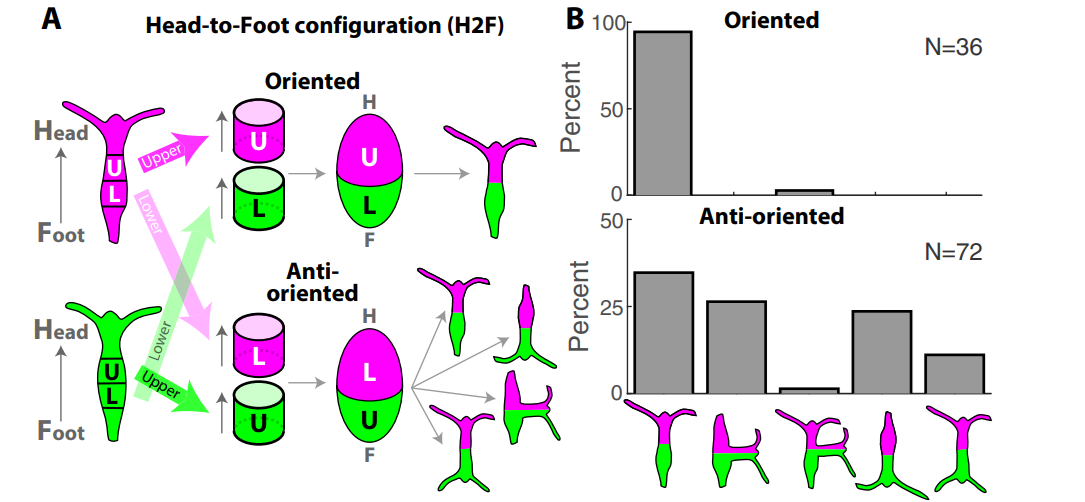
\includegraphics[
      width=0.94\textwidth,
      height=6.35cm,
      keepaspectratio
    ]{figures/E_growth_wound_and_sd/H2F.png}

    \vspace{0.14cm}

    {\color{HydraMuted}\fontsize{6}{7.2}\selectfont
      Livshits, Garion, Maroudas-Sacks, Shani-Zerbib, Keren \& Braun,
      \textit{Sci.\ Rep.} \textbf{12}:13368 (2022), Fig.~2A--B.\par}
  \end{center}

\end{frame}


% =============================================================================
% 3 -- Naming the missing quantity.
% =============================================================================
\begin{frame}{Missing ingredient}

  \vspace{-0.14cm}

  \begin{columns}[c,onlytextwidth]

    \begin{column}{0.40\textwidth}
      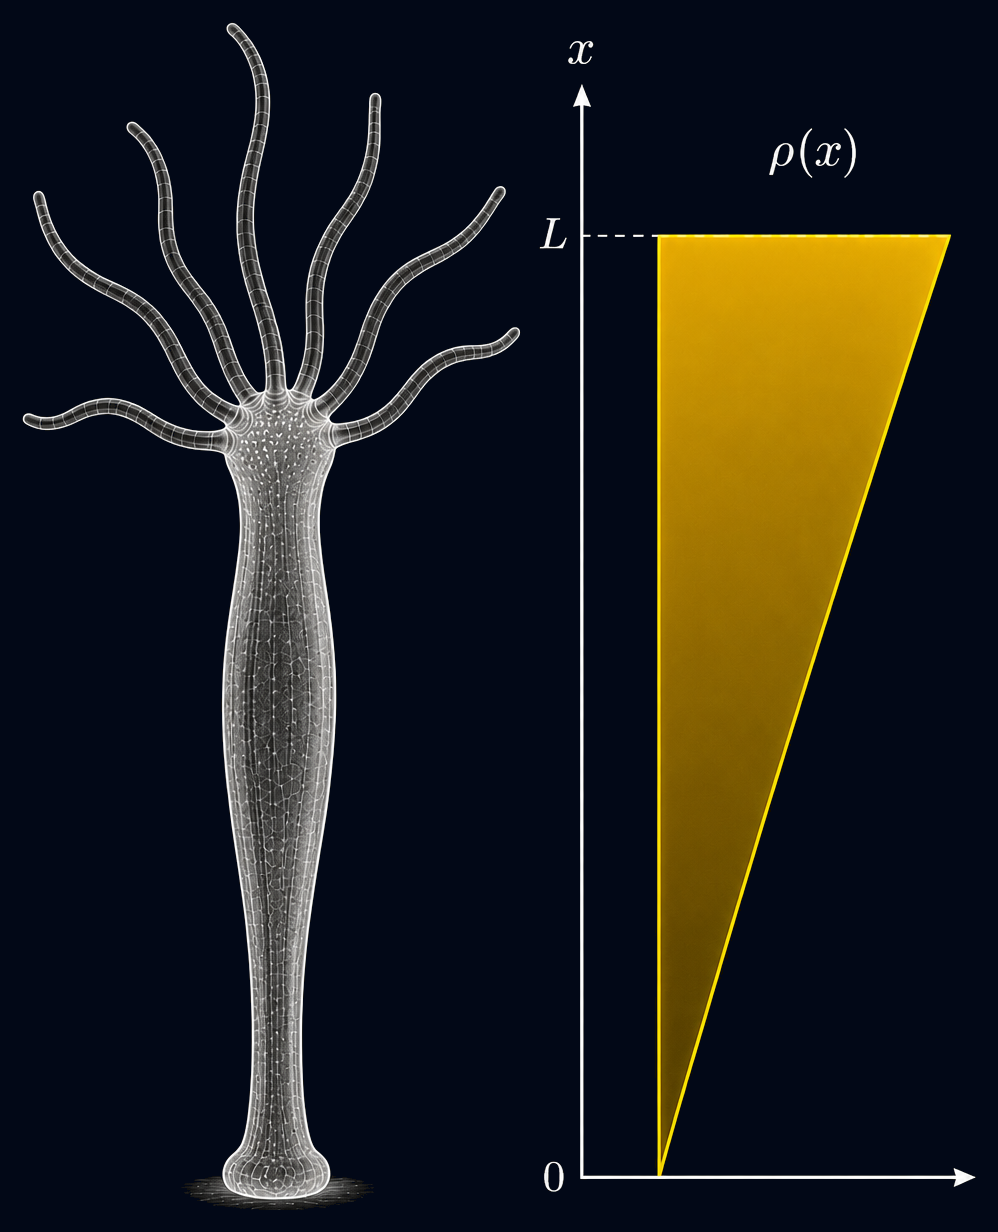
\includegraphics[
        width=\linewidth,
        height=5.45cm,
        keepaspectratio
      ]{figures/E_growth_wound_and_sd/rho_gradient.png}
    \end{column}

    \begin{column}{0.56\textwidth}

      \HydraPoint[HydraGold]
        {How do we tell two pieces of tissue apart?}
        {Nothing in the equations distinguishes tissue taken from near the head
         from tissue taken from near the foot.}

      \vspace{0.10cm}

      \HydraPoint[HydraCyan]
        {Positional information}
        {Each piece carries a memory of where it sat along the body axis of the
         parent animal.}

      \vspace{0.10cm}

      \HydraPoint[HydraGold]
        {$\rho(x)$ influences the production of both components}
        {The same graded factor multiplies the production of the activator and
         of the inhibitor.}

    \end{column}

  \end{columns}

\end{frame}


% =============================================================================
% 4 -- The model with rho(x).  Same numerical presentation as the model slide
% in the Gierer--Meinhardt section, so the new factor is the only difference
% the audience has to absorb.
% =============================================================================
\begin{frame}{Model with $\rho(x)$}

  \vspace{-0.30cm}

  \begin{columns}[c,onlytextwidth]

    \begin{column}{0.58\textwidth}

      {\color{HydraWhite}\fontsize{8.6}{10.6}\selectfont
      Let $\Omega=[0,1]\subset\mathbb R$ be an interval
      \par}

      \vspace{-0.34cm}

      {\color{HydraWhite}\fontsize{9.9}{12.6}\selectfont
      \begin{align*}
        \partial_tu
        &=
        0.01\Delta u
        +
        {\color{HydraGold}\rho(x)}\,
        \frac{1.5u^2}{1+v}
        -
        0.5u
        \\
        \partial_tv
        &=
        \Delta v
        +
        {\color{HydraGold}\rho(x)}\,
        2u^2
        -
        v
      \end{align*}
      }

      \vspace{-0.22cm}

      \HydraPoint[HydraCyan]
        {Initial conditions}
        {$u(x,0)=u_0(x)$ and $v(x,0)=v_0(x)$}

      \vspace{-0.14cm}

      \HydraPoint[HydraGold]
        {No-flux boundaries}
        {$\partial_x u(x,t)=\partial_x v(x,t)=0$ at $x=0$ and $x=1$}

    \end{column}

    \begin{column}{0.38\textwidth}
      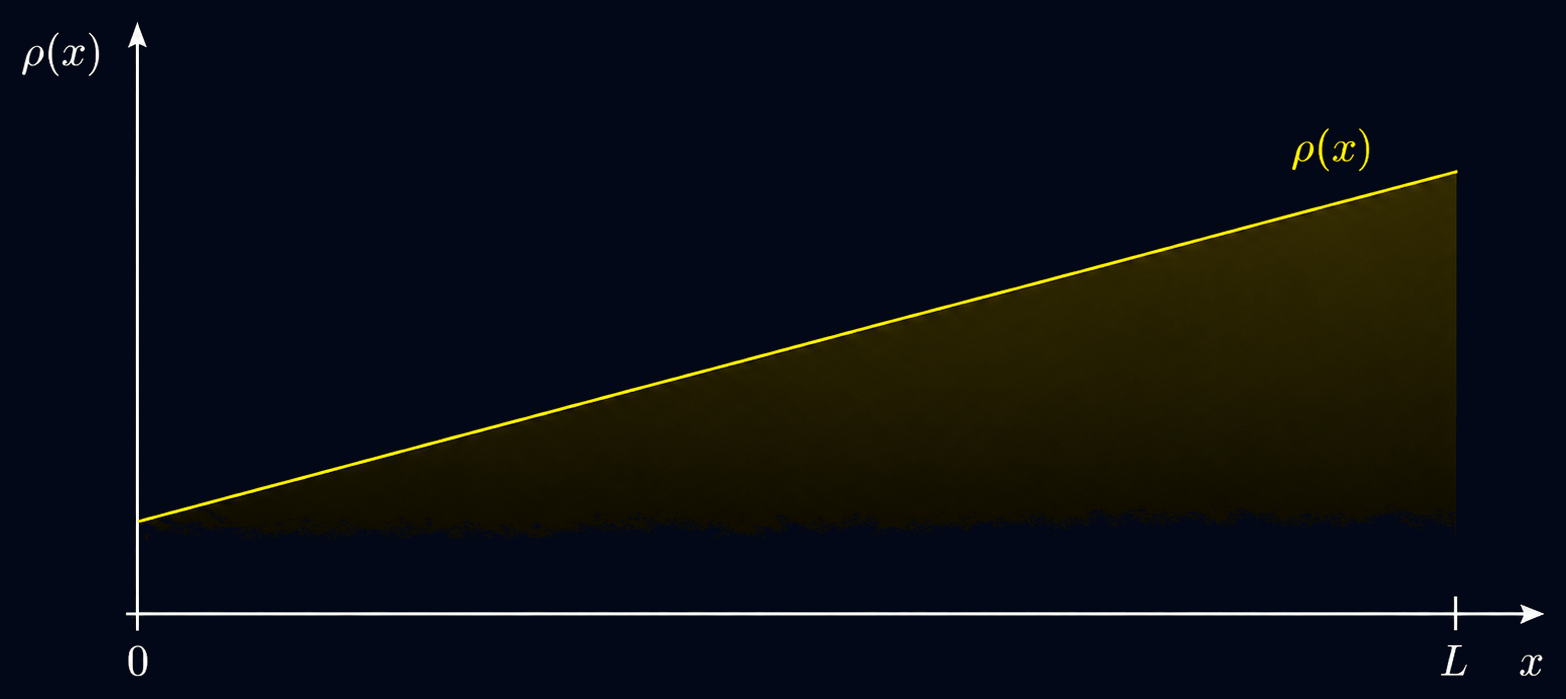
\includegraphics[
        width=\linewidth,
        height=3.30cm,
        keepaspectratio
      ]{figures/E_growth_wound_and_sd/rho_linear.png}
    \end{column}

  \end{columns}

  \vspace{0.24cm}

  \begin{columns}[T,onlytextwidth]

    \begin{column}{0.31\textwidth}
      {\color{HydraWhite}\bfseries\fontsize{8.0}{9.8}\selectfont
        Hard to analyse\par}
      \vspace{-0.04cm}
      {\color{HydraBody}\fontsize{6.6}{8.3}\selectfont
        A space-dependent coefficient breaks the tools built up so far.\par}
    \end{column}

    \begin{column}{0.31\textwidth}
      {\color{HydraWhite}\bfseries\fontsize{8.0}{9.8}\selectfont
        No positive constant steady state\par}
      \vspace{-0.04cm}
      {\color{HydraBody}\fontsize{6.6}{8.3}\selectfont
        Only the trivial state survives, and every earlier section
        linearised about a positive one.\par}
    \end{column}

    \begin{column}{0.31\textwidth}
      {\color{HydraWhite}\bfseries\fontsize{8.0}{9.8}\selectfont
        Theory exists, but it is heavy\par}
      \vspace{-0.04cm}
      {\color{HydraBody}\fontsize{6.6}{8.3}\selectfont
        Rigorous results are available and considerably more involved.\par}
    \end{column}

  \end{columns}

\end{frame}




% =============================================================================
% 6 -- The objection that forces the rest of the section.
% =============================================================================
\begin{frame}{But where does $\rho(x)$ come from?}

  \vspace{0.20cm}

  \HydraPoint[HydraGold]
    {It is put in by hand}
    {We chose the profile ourselves. Nothing in the model produces it.}

  \vspace{0.14cm}

  \HydraPoint[HydraCyan]
    {It never changes}
    {A prescribed $\rho(x)$ is fixed for all time, so the tissue cannot
     rewrite what it knows about its own position.}

  \vspace{0.14cm}

  \HydraPoint[HydraGold]
    {Regeneration has to restore it}
    {The animal that grows back must carry a proper gradient again, ready
     for the next cut. A prescribed profile offers no mechanism for that.}

  \vspace{0.30cm}

  \HydraTakeaway{
    If the source density matters, it has to be a variable of the model
  }

\end{frame}


% =============================================================================
% 7 -- Promoting rho to a variable.  No time scale yet: the equation relaxes
% as fast as everything else.
% =============================================================================
\begin{frame}{Source density as a variable}

  \vspace{-0.16cm}

  \begin{columns}[c,onlytextwidth]

    \begin{column}{0.46\textwidth}

      {\color{HydraWhite}\fontsize{10.2}{13}\selectfont
      \begin{align*}
        \partial_t\rho
        &=
        D_{\rho}\Delta\rho
        +
        u
        -
        \rho
      \end{align*}
      }

      \vspace{-0.20cm}

      {\color{HydraMuted}\fontsize{7.4}{9.1}\selectfont
        with $\partial_x\rho=0$ at $x=0$ and $x=1$
      \par}

      \vspace{0.34cm}

      \HydraPoint[HydraCyan]
        {The activator writes it}
        {Wherever the activator is high, the tissue becomes better at
         producing it.}

      \vspace{0.06cm}

      \HydraPoint[HydraGold]
        {Diffusion spreads it out}
        {$D_{SD}$ turns a sharp peak into a profile that varies across the
         whole domain.}

    \end{column}

    \begin{column}{0.50\textwidth}
      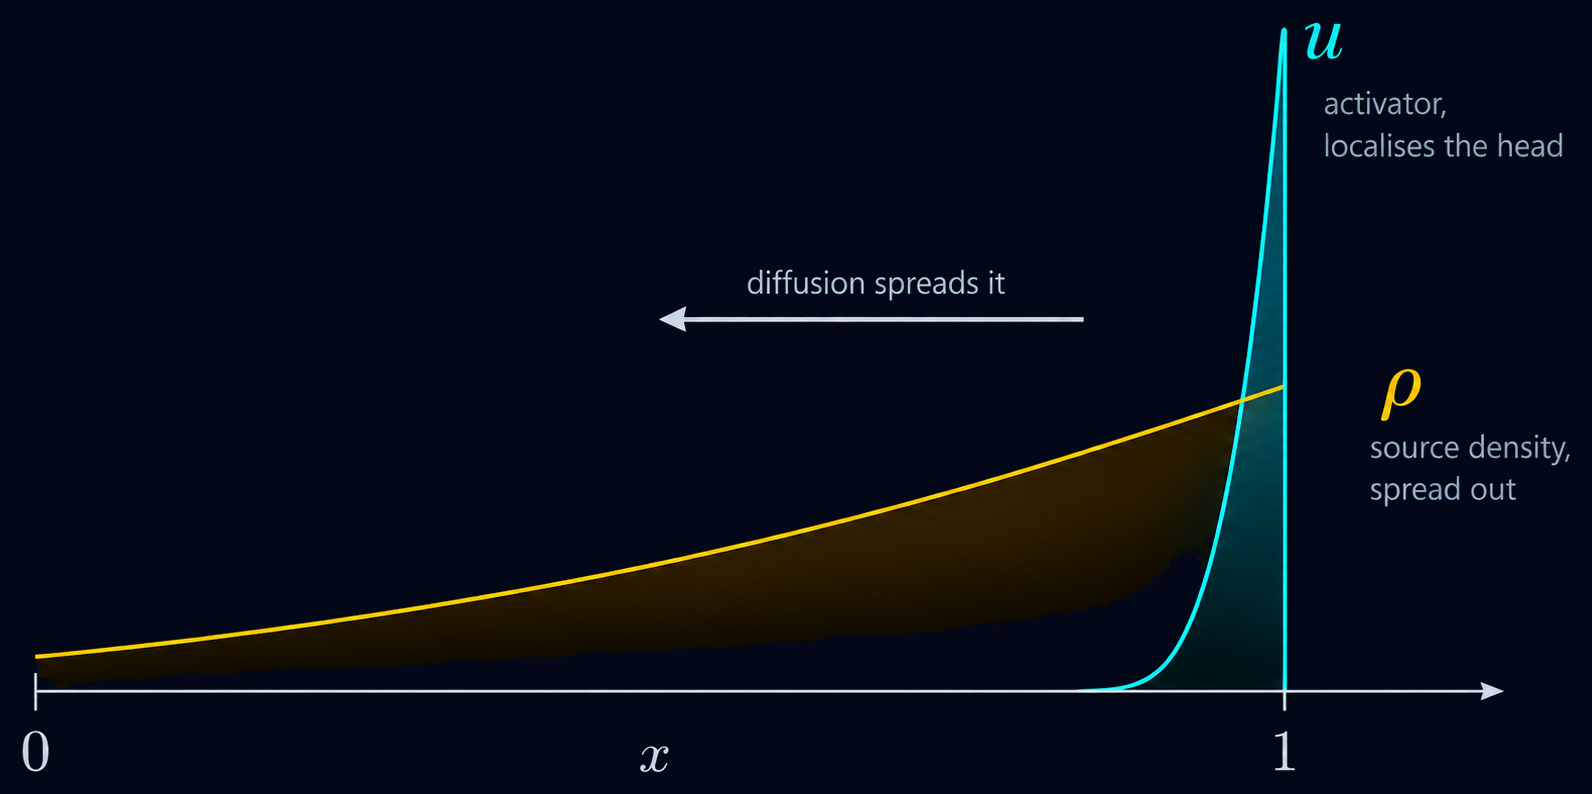
\includegraphics[
        width=\linewidth,
        height=4.75cm,
        keepaspectratio
      ]{figures/E_growth_wound_and_sd/rho_spreading.png}
    \end{column}

  \end{columns}

\end{frame}


% =============================================================================
% 8 -- What the analysis does and does not change.
% =============================================================================
\begin{frame}{The analysis survives, at a price}

  \vspace{-0.24cm}

  {\color{HydraWhite}\fontsize{9.7}{12.3}\selectfont
  \begin{align*}
    \partial_tu
    &=
    0.01\Delta u
    +
    \rho\,\frac{1.5u^2}{1+v}
    -
    0.5u
    \\
    \partial_tv
    &=
    \Delta v
    +
    \rho\,2u^2
    -
    v
    \\
    \partial_t\rho
    &=
    D_{SD}\Delta\rho
    +
    u
    -
    \rho
  \end{align*}
  }

  \vspace{0.20cm}

  \begin{columns}[T,onlytextwidth]

    \begin{column}{0.47\textwidth}
      \HydraPoint[HydraCyan]
        {More computation}
        {Three components instead of two: the characteristic polynomial is
         cubic and the algebra grows accordingly.}
    \end{column}

    \begin{column}{0.47\textwidth}
      \HydraPoint[HydraGold]
        {Similar criteria}
        {Turing instability appears in the same way, and the conditions for it
         look much as before.}
    \end{column}

  \end{columns}

\end{frame}


% =============================================================================
% 9 -- The simulation that shows the promotion was empty.
% =============================================================================
\begin{frame}{A variable that forgets as fast as it learns}

  \vspace{-0.06cm}

  \SDLive[4.55cm]{Run the three-component system with \mbox{$\tau=1$} and watch the source density track the activator instead of outliving it}

  \vspace{0.16cm}

  \HydraTakeaway{
    Making $\rho$ a variable bought us nothing, because it relaxes as
    quickly as the pattern that writes it
  }

\end{frame}


% =============================================================================
% 10 -- The time scale.  This is the point of the whole section.
% =============================================================================
\begin{frame}{Adding a time scale}

  \vspace{-0.10cm}

  \begin{center}
    {\color{HydraWhite}\fontsize{11.4}{14.4}\selectfont
    \begin{align*}
      {\color{HydraGold}\tau}\,\partial_t\rho
      &=
      D_{\rho}\Delta\rho
      +
      u
      -
      \rho
    \end{align*}
    }
  \end{center}

  \vspace{0.16cm}

  \begin{columns}[T,onlytextwidth]

    \begin{column}{0.31\textwidth}
      \HydraPoint[HydraGold]
        {Memory}
        {Large $\tau$ makes the source density outlive the pattern that
         created it.}
    \end{column}

    \begin{column}{0.31\textwidth}
      \HydraPoint[HydraCyan]
        {Separation of scales}
        {The activator and inhibitor settle while $\rho$ is still almost
         frozen.}
    \end{column}

    \begin{column}{0.31\textwidth}
      \HydraPoint[HydraGold]
        {The prescribed profile returns}
        {As $\tau$ grows, the model approaches the fixed $\rho(x)$ we started
         with, now as a limit rather than an assumption.}
    \end{column}

  \end{columns}

  \vspace{0.28cm}

  \HydraTakeaway{
    $\tau$ does not decide whether a pattern forms, but how long the tissue
    remembers where it was
  }

\end{frame}


% =============================================================================
% 11 -- What the finished model does.
% =============================================================================
\begin{frame}{Model with source density}

  \vspace{-0.06cm}

  \SDLive[4.65cm]{Run the same system with a slow source density and watch the gradient be inherited, rewritten, and set the site of the new head}

  \vspace{0.16cm}

  \HydraTakeaway{
    The gradient is no longer assumed, the tissue writes it, keeps it, and
    hands it on
  }

\end{frame}

\PerfectModel

\begin{frame}{Recall the Gierer--Meinhardt mechanism}

  \vspace{-0.32cm}

  \begin{columns}[c,onlytextwidth]
    \begin{column}{0.57\textwidth}
      {\color{HydraMuted}\fontsize{7.6}{9.3}\selectfont
        The chemical mechanism uses two interacting substances
      \par}

      \vspace{-0.30cm}

      {\color{HydraWhite}\fontsize{9.5}{12}\selectfont
      \begin{align*}
        \partial_tu
        &=D_u\Delta u+\frac{au^2}{K+v}-\mu_u u
        \\
        \partial_tv
        &=D_v\Delta v+bu^2-\mu_v v
      \end{align*}
      }

      \vspace{-0.40cm}

      \HydraPoint[HydraGold]
        {Local activation}
        {The activator promotes its own production over a short range}

      \vspace{-0.10cm}

      \HydraPoint[HydraCyan]
        {Long-range inhibition}
        {A second substance suppresses activation over a larger spatial scale}
    \end{column}

    \begin{column}{0.39\textwidth}
      \centering
      \begin{tikzpicture}[x=0.88cm,y=0.88cm]
        \draw[HydraLine,line width=1.0pt] (0.45,2.65) -- (5.35,2.65);
        \fill[HydraGold] (2.90,2.65) circle[radius=0.16cm];
        \fill[HydraGold,opacity=0.48] (2.35,2.65) circle[radius=0.10cm];
        \fill[HydraGold,opacity=0.48] (3.45,2.65) circle[radius=0.10cm];
        \draw[<->,HydraGold,line width=1.1pt] (2.25,3.30) -- (3.55,3.30);
        \node[text=HydraGold,font=\bfseries\fontsize{7.2}{8.6}\selectfont]
          at (2.90,3.68) {activation};
        \draw[<->,HydraCyan,line width=1.1pt] (0.75,1.78) -- (5.05,1.78);
        \node[text=HydraCyan,font=\bfseries\fontsize{7.2}{8.6}\selectfont]
          at (2.90,1.34) {inhibition};
        \node[text=HydraMuted,align=center,text width=4.6cm,
          font=\fontsize{7}{8.5}\selectfont]
          at (2.90,0.55) {two spatial scales are encoded by two diffusible substances};
      \end{tikzpicture}
    \end{column}
  \end{columns}

\end{frame}


\begin{frame}{The activator has candidates but the inhibitor remains unclear}

  \vspace{-0.12cm}

  \begin{columns}[c,onlytextwidth]
    \begin{column}{0.47\textwidth}
      \centering
      {\color{HydraGold}\bfseries\fontsize{8}{9.5}\selectfont
        ACTIVATOR CANDIDATE\par}
      \vspace{0.22cm}
      {\color{HydraWhite}\bfseries\fontsize{21}{24}\selectfont Wnt3\par}
      \vspace{0.22cm}
      {\color{HydraMuted}\fontsize{7.5}{9.2}\selectfont
        Stable localized Wnt3 expression marks the emerging head organizer
      \par}
    \end{column}

    \begin{column}{0.06\textwidth}
      \centering{\color{HydraLine}\fontsize{28}{28}\selectfont $\vert$}
    \end{column}

    \begin{column}{0.47\textwidth}
      \centering
      {\color{HydraCyan}\bfseries\fontsize{8}{9.5}\selectfont
        MISSING COMPONENT\par}
      \vspace{0.22cm}
      {\color{HydraWhite}\bfseries\fontsize{18}{22}\selectfont ?\par}
      \vspace{0.22cm}
      {\color{HydraMuted}\fontsize{7.5}{9.2}\selectfont
        No biochemical species has been established as the required fast long-range inhibitor
      \par}
    \end{column}
  \end{columns}

  \vspace{0.48cm}

  \HydraTakeaway{
    The mathematical inhibitor has a clear role but its biological identity is unresolved
  }

\end{frame}